\chapter{Introduction to Medical Image Analysis}
\label{sec:chap2}

\section{Motivation}
A \textbf{tumor} is an abnormal mass of tissue that forms when cells grow and divide unusually. Tumors are divided into two main categories: benign (not cancer) or malignant (cancer). Benign tumors may grow large but do not invade other parts of the body.  On the other hand, malignant tumors can spread into nearby tissues.

There are different reasons for creating tumors; the first reason is the body tissue near the tumor area. But in some cases, it is brought from other parts of the body. The risk level of tumors depends on four factors: 

\begin{enumerate}
	\item Type of the tumor (benign or malignant)
	\item Size of tumor
	\item Location of tumor
	\item Speed of tumor spread
\end{enumerate}

In recent years, the improvement of medical imaging techniques helps doctors to diagnose tumors. Imaging tests are used to determine the size and location of cancer. Medical imaging is a technique and process to build a picture of the whole human body or a part of it for medical purposes. 

Early detection of tumors will increase the chance of treatment and plays an essential role in patient survival. On the other hand, manual tumor segmentation (by an expert) among a large number of medical images could be hard and time-consuming.  Also, it depends on the experience of the expert who does this segmentation. Therefore, we need a completely automated and precise approach to segment and detect tumors. Recently, using image processing and machine learning methods has become common due to their promising results. 

A thorough analysis of the literature with the keywords ‘brain tumor segmentation’, ‘medical image segmentation machine learning’, and ‘medical image analysis deep learning’ on the Google Scholar search engine is performed in Fig. \ref{fig1}, queried on August 16, 2021. We can observe that the number of papers increases every year from 2013 to 2021, which means multi-modal medical image segmentation using machine learning, and deep learning are obtaining more and more attention in recent years. 

\begin{figure}[h]
	\centering
	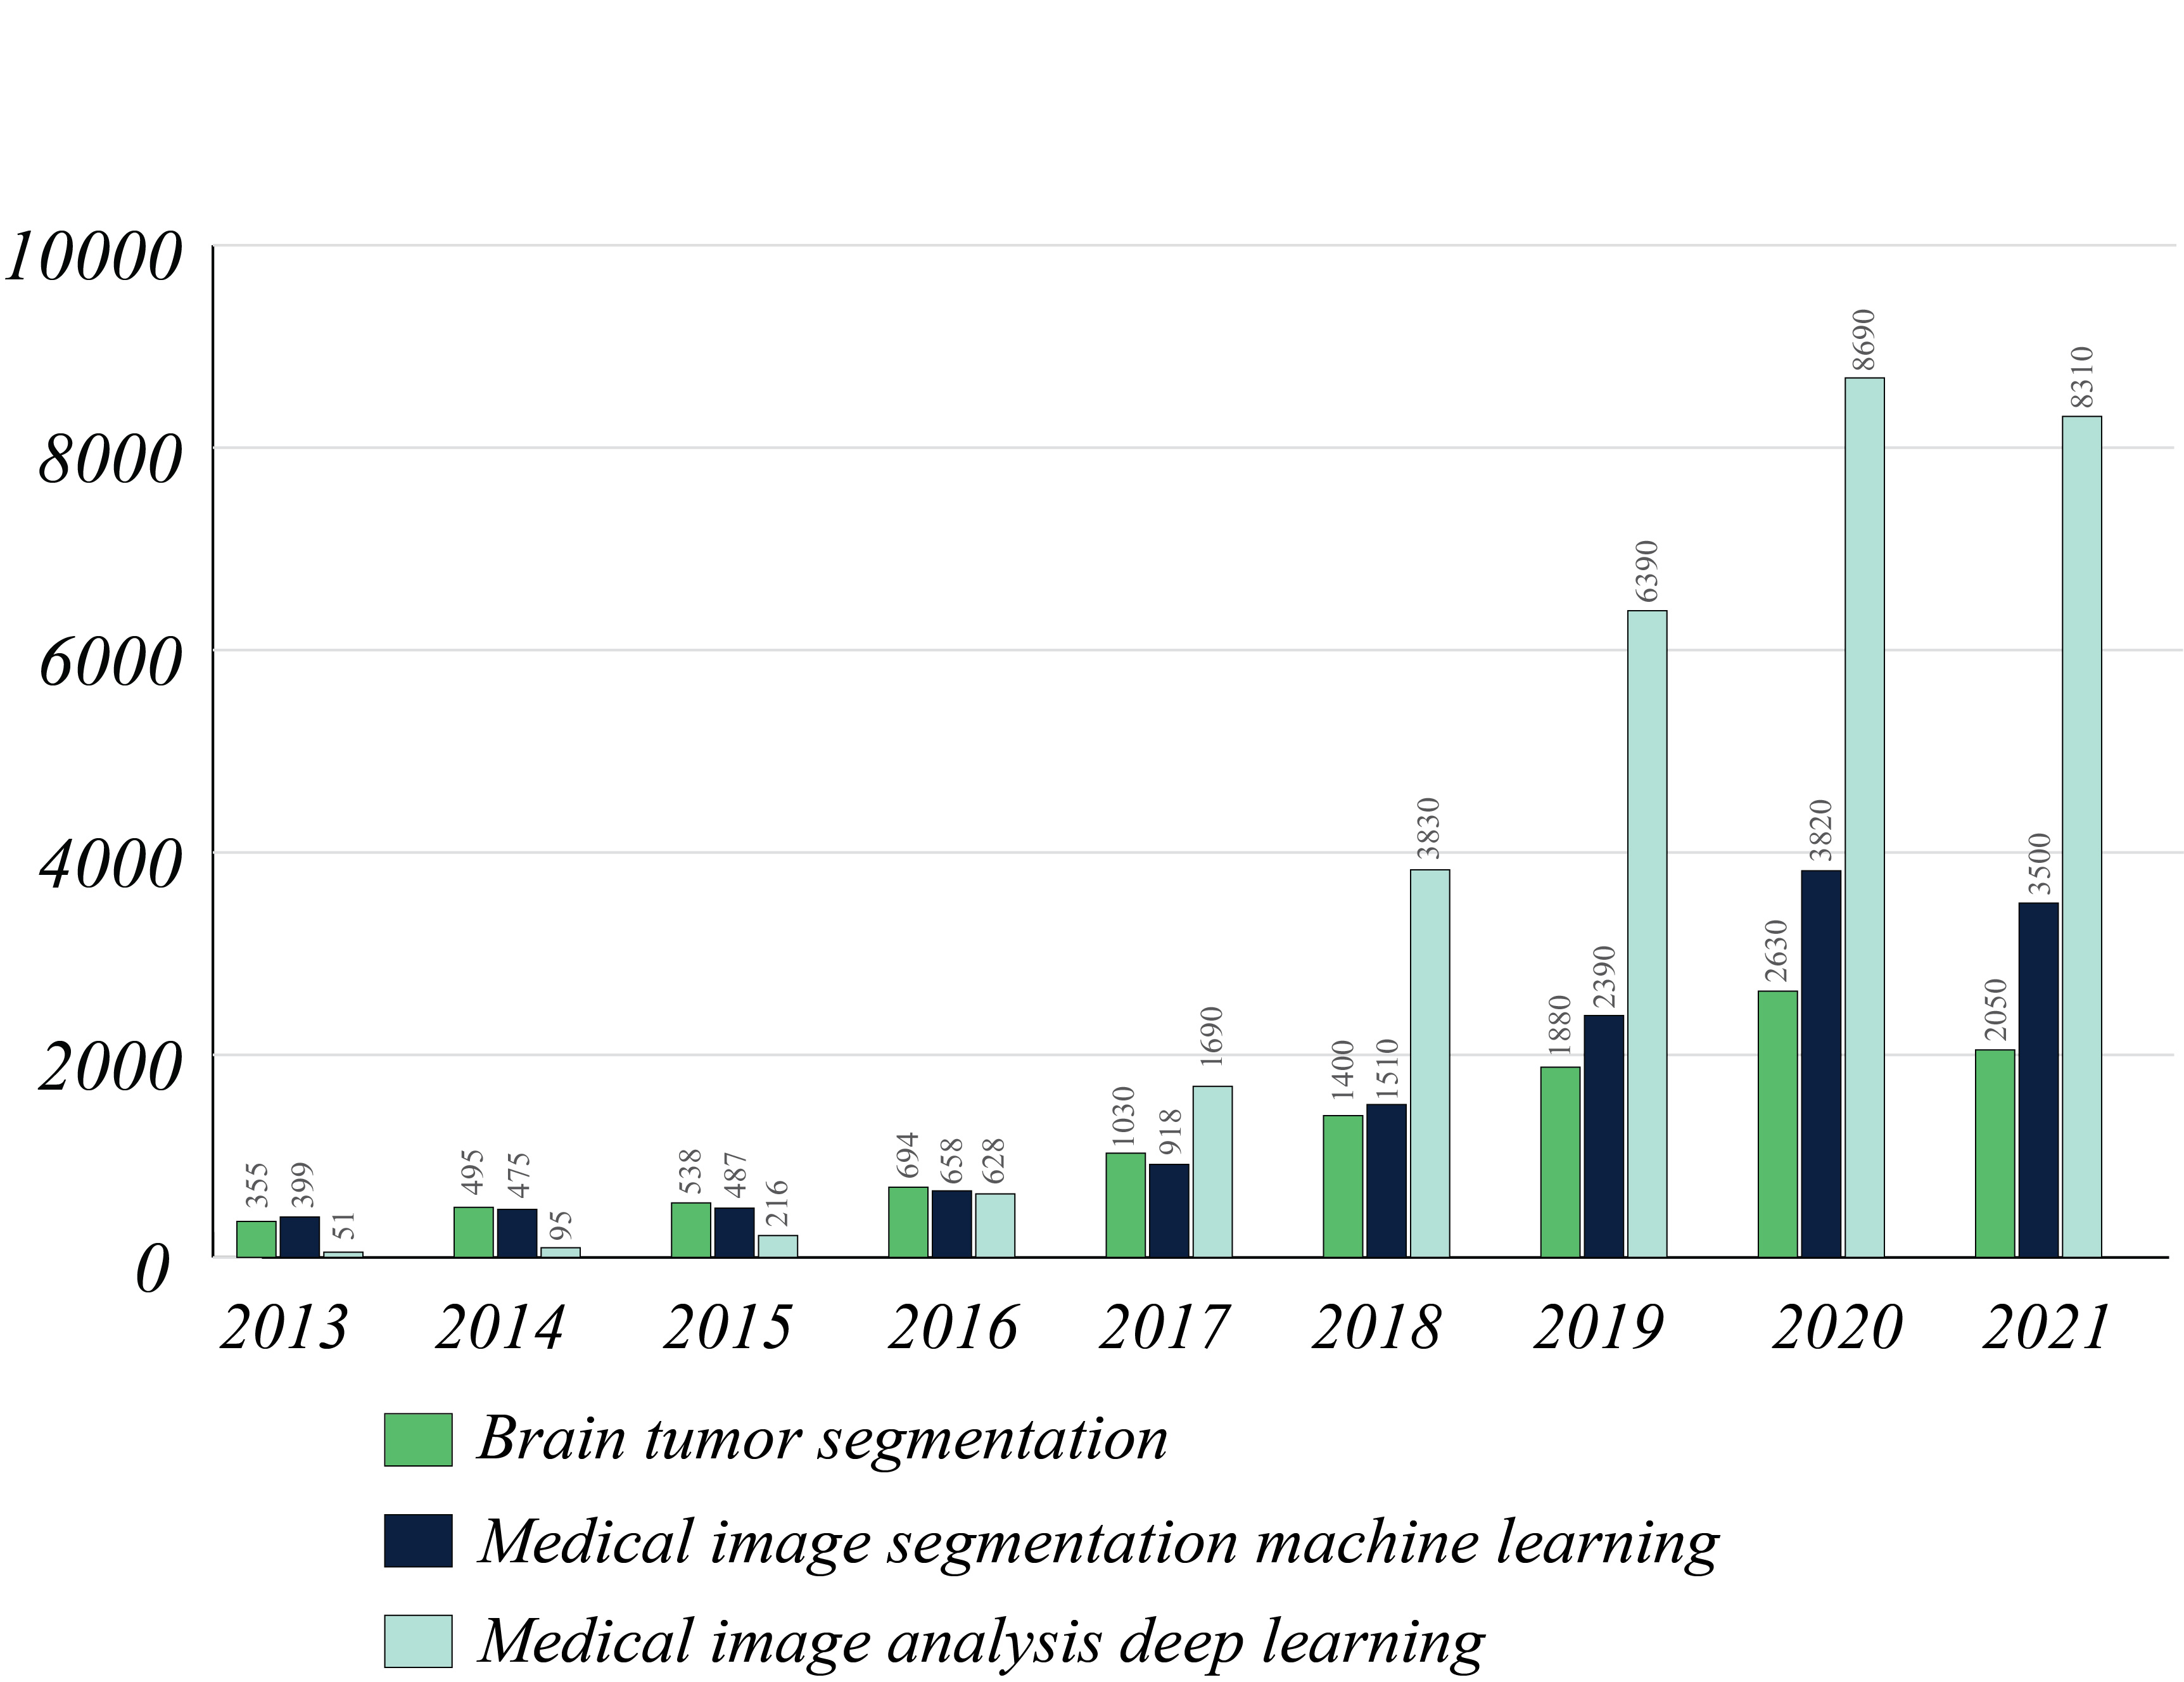
\includegraphics[width=1\columnwidth]{./figures/Fig1.jpg}
	\caption{Keywords search results}
	\label{fig1}
\end{figure}

\section{what is medical image analysis}

In 2020, the whole machine vision market was worth about 12.29 billion dollars, and out of this, 39\% of the total share would be what will be taken down by medical image analysis itself. It will not be focused on hospitals or private health care centers or any particular modality like x-ray or ultrasound. So we can use it in different modalities, clinical indications, and different end-users. Figure \ref{fig2} illustrates the concepts and applications of medical image analysis.

\begin{figure}[h]
	%\resizebox{\linewidth}{!}{
	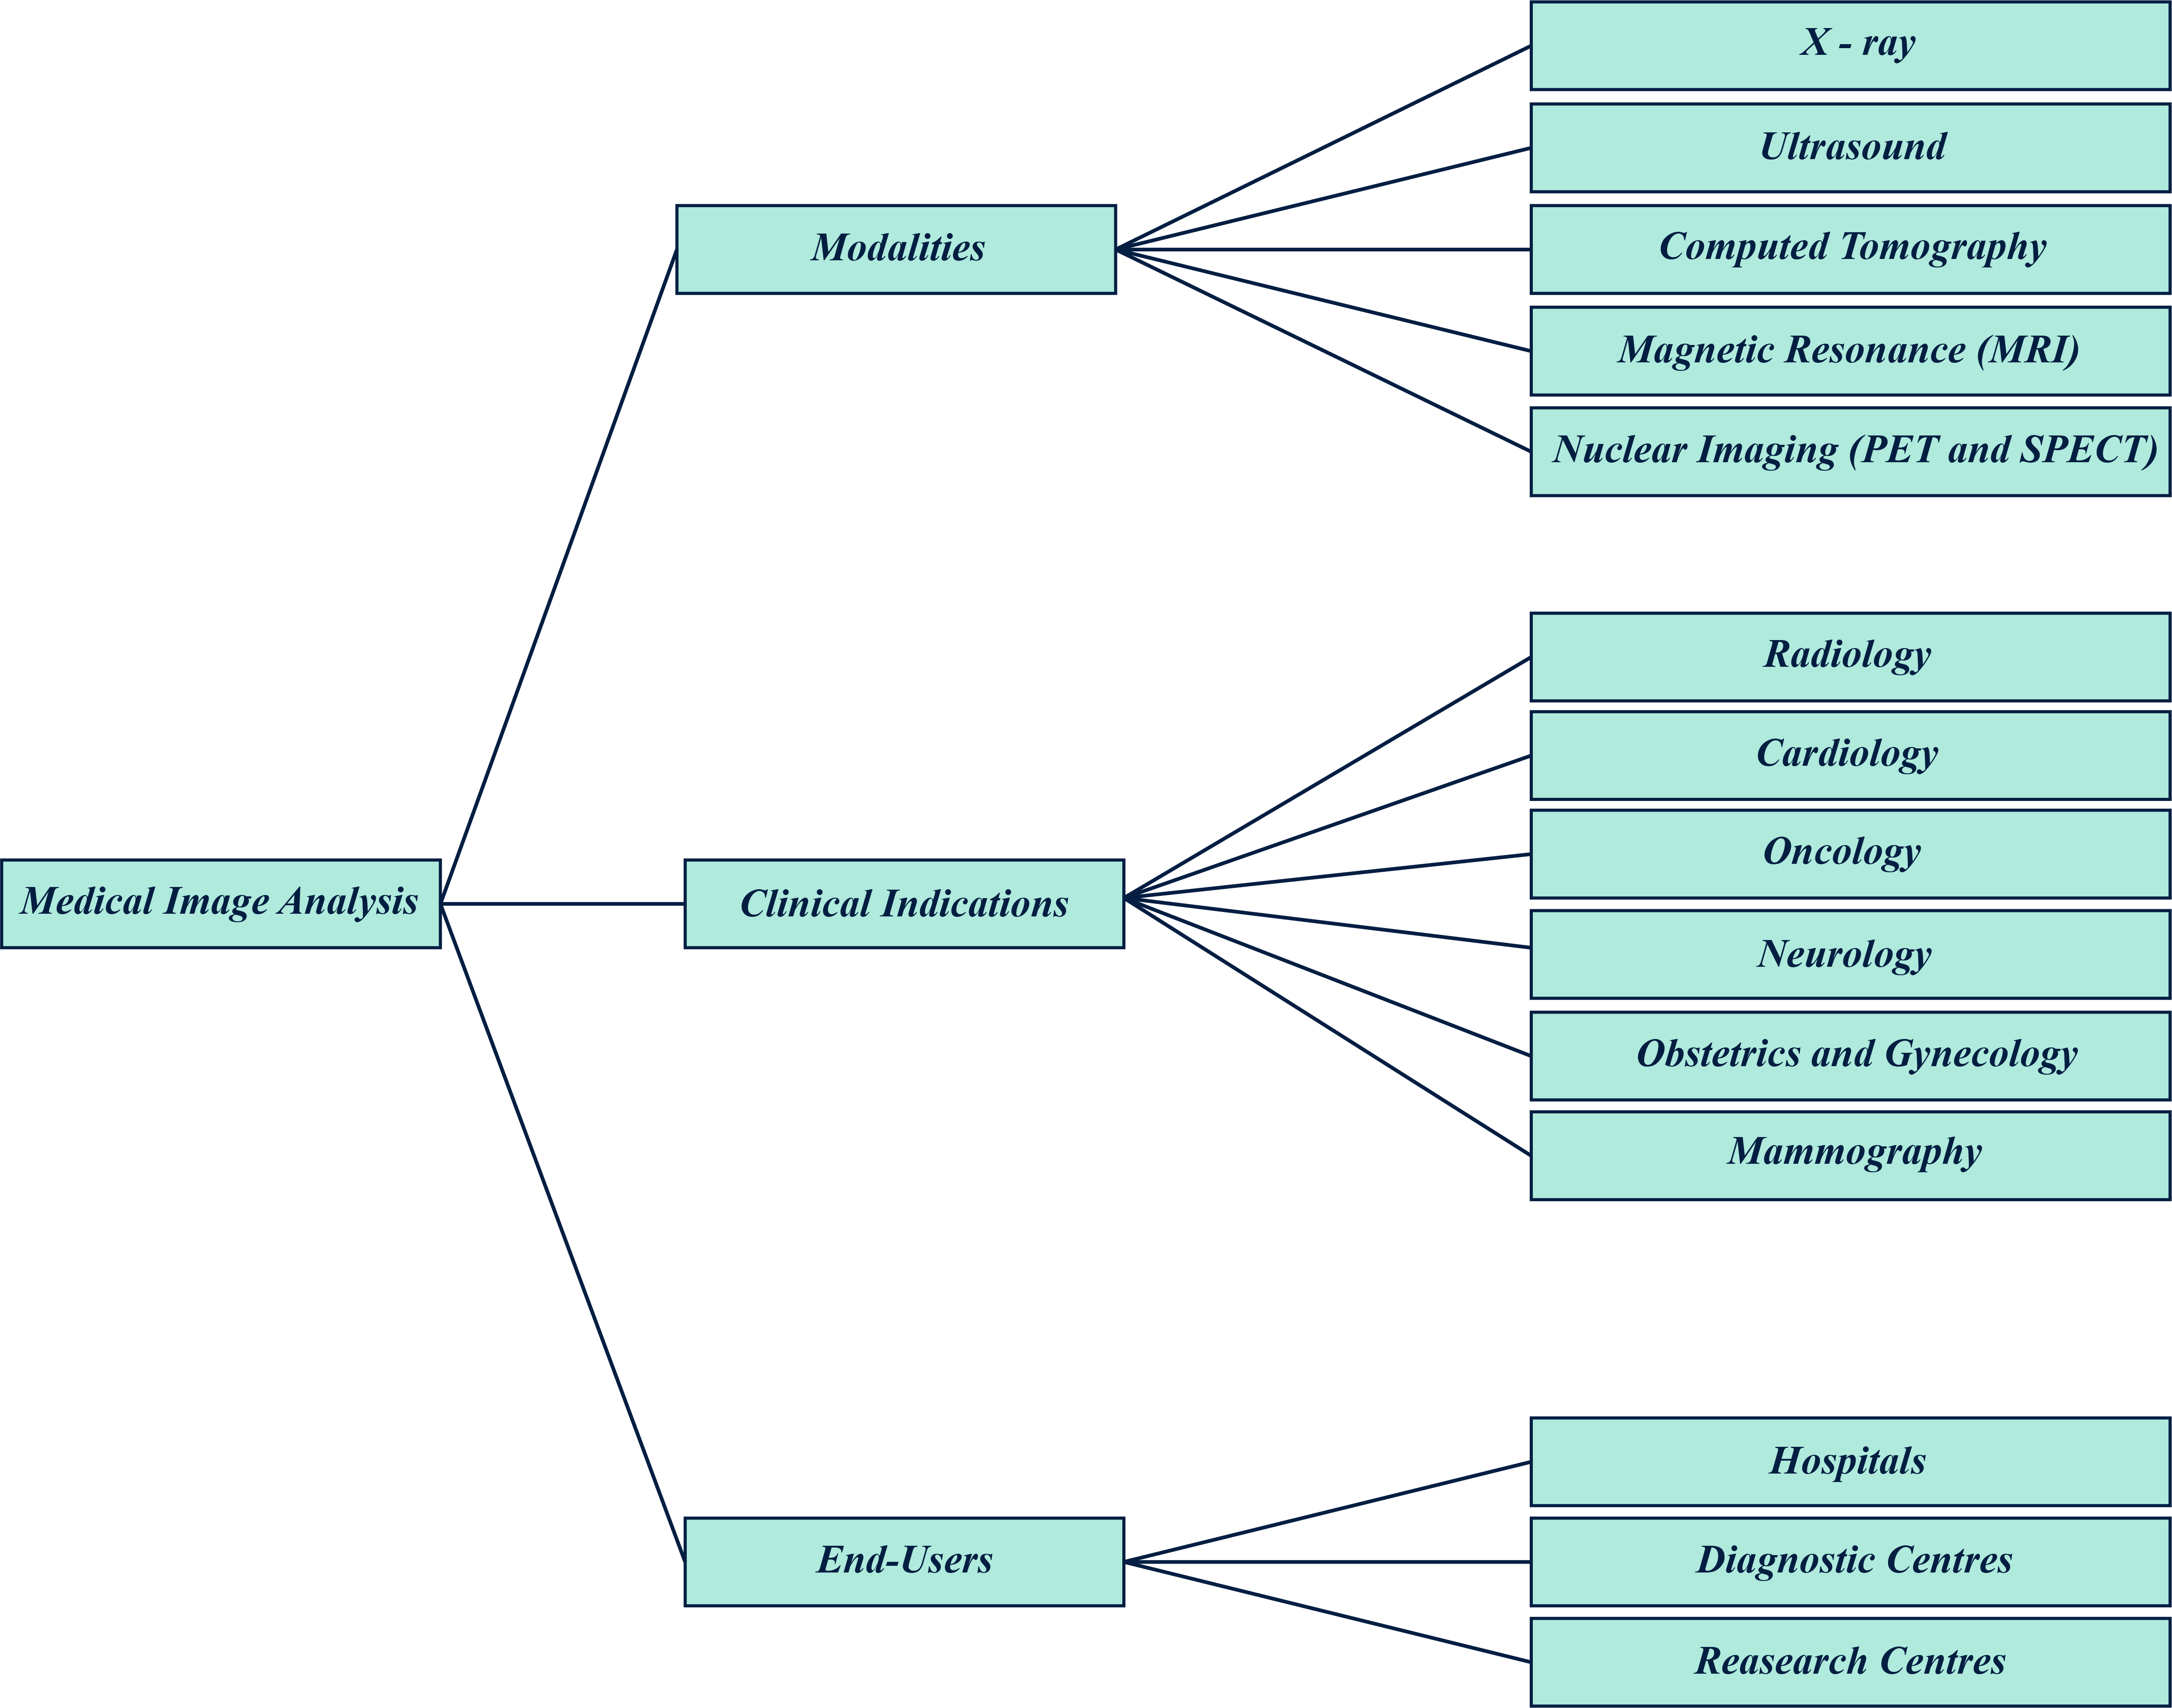
\includegraphics[width=1\columnwidth]{./figures/Fig2.png}
	\caption{Medical image analysis (concepts and applications)}
	\label{fig2}
\end{figure}

\section{roadmap}


If we look into different modalities such as CT, MRI, ultrasound, etc. The critical part is about the organ appearance module and what they mean. In other words, how different organs are going to appear in different modalities. For example, a bone will appear brighter on x-rays, and it would be darker on T1 MR and T2 MR. On the other hand, fatty regions appear brighter on MR and darker on x-rays; fatty areas will appear brighter on ultrasound. A water-filled part that would appear brighter on MR will appear darker on ultrasound.

The second part for understanding medical image processing is to understand the physics part of it. As we mentioned above, different parts of the body have different ways in which they are viewed, and it is where we need to understand tissue energy interactions together. And from there, image formation and statistics of image formation will get vital because we will see a lot of noise and uncertainty. For example, ultrasound is a specular modality that has a lot of jitters and noise around intensities.
On the other hand, MRI will not have that much problem, but it suffers from lower resolution than ultrasound, and when we go into detail understanding of each of this physics and how operating conditions of an instrument affects the total resolution of image formation.

After medical imaging and physics, we would be moving on to image processing and graphics in the third step. Image processing is an essential part of medical image analysis because it contains Denoising, feature segmentation, image segmentation, and feature representation. After that, we got onto a very critical factor called visualization. Also, knowledge of graphics is fundamental. 

Last but not least is machine learning which has grown in recent years. Machine learning includes prediction models and a group of classifiers. We can use various methods to solve a particular problem, such as example-based learning methods or complex reasoning. So to conclude these four main steps of medical image processing, we bring them as Figure \ref{fig3}.

\begin{figure}[h]
	%\resizebox{\linewidth}{!}{
	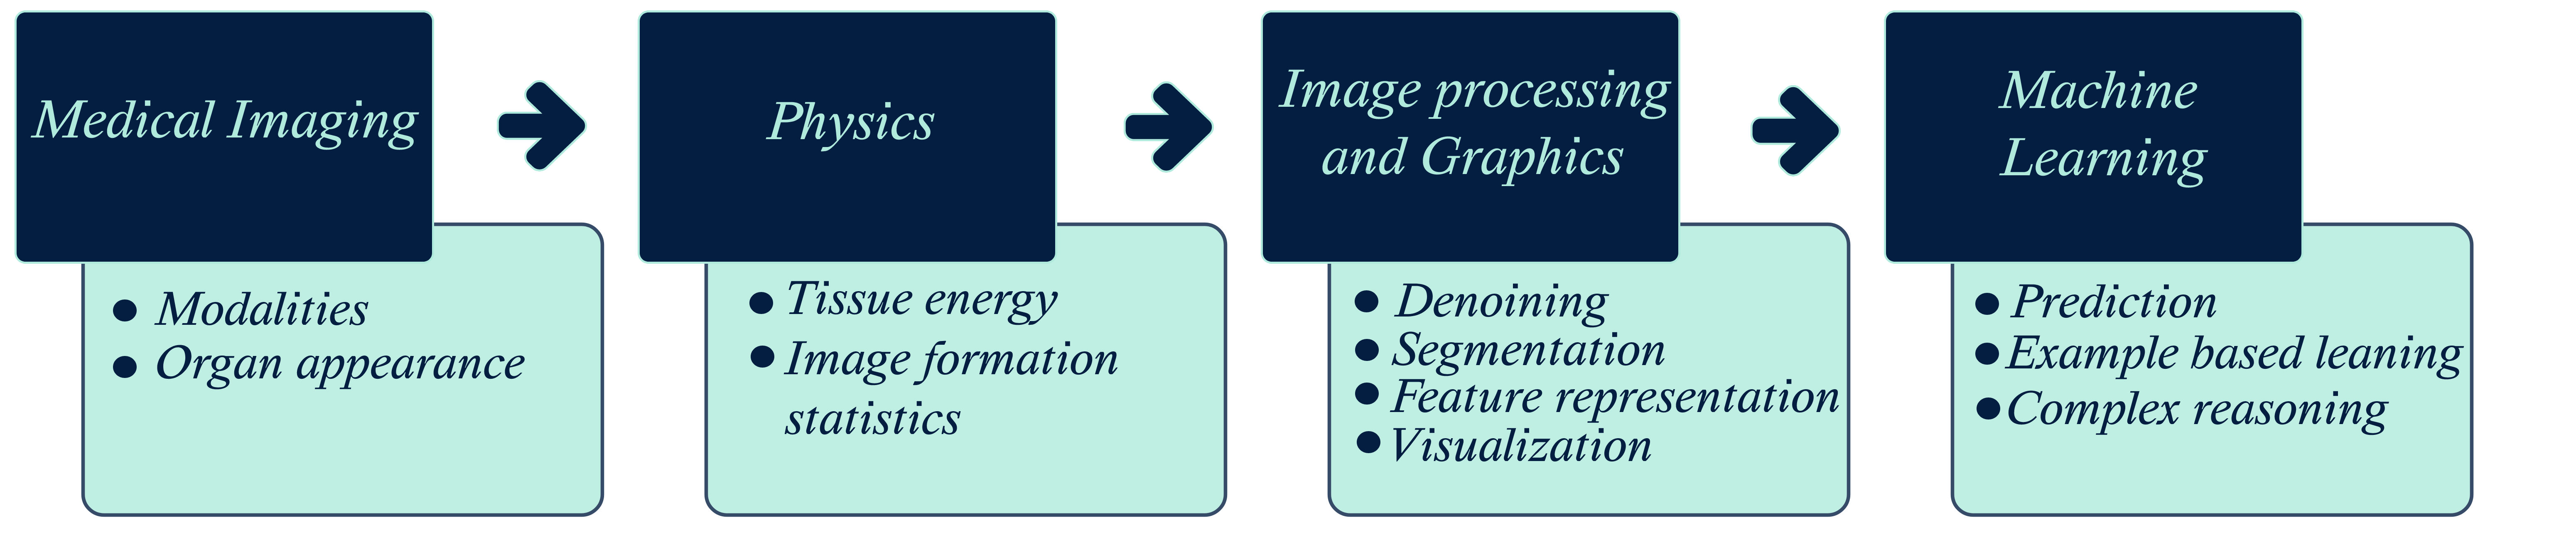
\includegraphics[width=1\columnwidth]{./figures/Fig3.png}
	\caption{Medical image analysis roadmap}
	\label{fig3}
\end{figure}

\section{research and business areas}

Let us look into the main areas of research and business that medical image analysis is concerned. The first one is the range of image modalities which are macro and micro imaging. Macro imaging is the method that the whole body gets imaged together, and obviously, the resolution is much lower, but the penetration depth is much higher. On the other hand, micro imaging has resolution at the microns' level and is used in some modalities like optical coherence, tomography, and histopathology for digital pathology. But, there is a tradeoff for scaling, and it is mesoscopic range imaging.

The second main area is image registration, a classical area for medical image analysis, and it says a patient goes for a CT scan. After six months, he or she does this again but at a different location and different CT machine. The resolutions are different because the patient might have a body change, such as losing some weight. The doctor wants actually to relate to what happened in the last six months. 

Another exciting area is organ localization which is where we need to find out the organ itself. This area uses algorithms to make it much easier for clinicians than wasting a lot of time. Also, As you know, we imaging in 3D, but you see the output on your computer screen or x-ray films which present only 2D pictures. Organ localization tries to use algorithms in 3D and segment them. After organ localization has been over, you can segment out and get the volume information and surface information.

In recent years, the research on visualization using augmented reality has been expanded. This area is related to present how different kinds of fractures can be there on a bone and then try to find out what the bone would look like without any fractures. 

Another interesting field is virtual anatomy, and it comes after we have a complete MR or CT scan of a patient body. The whole anatomy, such as every organ and every tissue or bone, is digitized and segmented using virtual anatomy. In other words, the body is equivalent to a computer-aided design (CAD) model. For example, if a doctor wants to find out internal injuries, specific legions, or diseases within the patient's body, they do not need to scan every x-ray.  

A very critical application in this area is digital angiography which is also called digital subtraction angiography. It is a technique to find out where is a deposition of blood or regularity inflow of blood.  
Despeakling is related to speckle imaging modalities like optical coherence or ultrasonic tomography, where many speckles lead to tediousness. This situation cannot just be Denoising because it would get rid of edges and salient behaviors. 


3D optical microscopy is a 3d model of a neuron image under fluorescence for different layers, segmented and resynthesized by alignment. We can look at the complete 3D model and view how neurons look and how the processes are going over there. This area has a significant role in a field of medicine called precision medicine. 

Digital pathology is the next critical area. With the help of pathology, the pathologist doesn't need to be at the center where the slide comes down. So say there is a collection center that is far from the actual pathologist is located. Transporting a physical slide takes more time and money, but digital pathology solved this problem. 

The last area in this section is computational imaging. Computational imaging is about synthesizing virtual equivalents of different organ types of different pathology types by looking at simple images and simple signals from image modalities. You can see all these areas in Figure \ref{fig4} .


\begin{figure}[htbp]
	%\resizebox{\linewidth}{!}{
	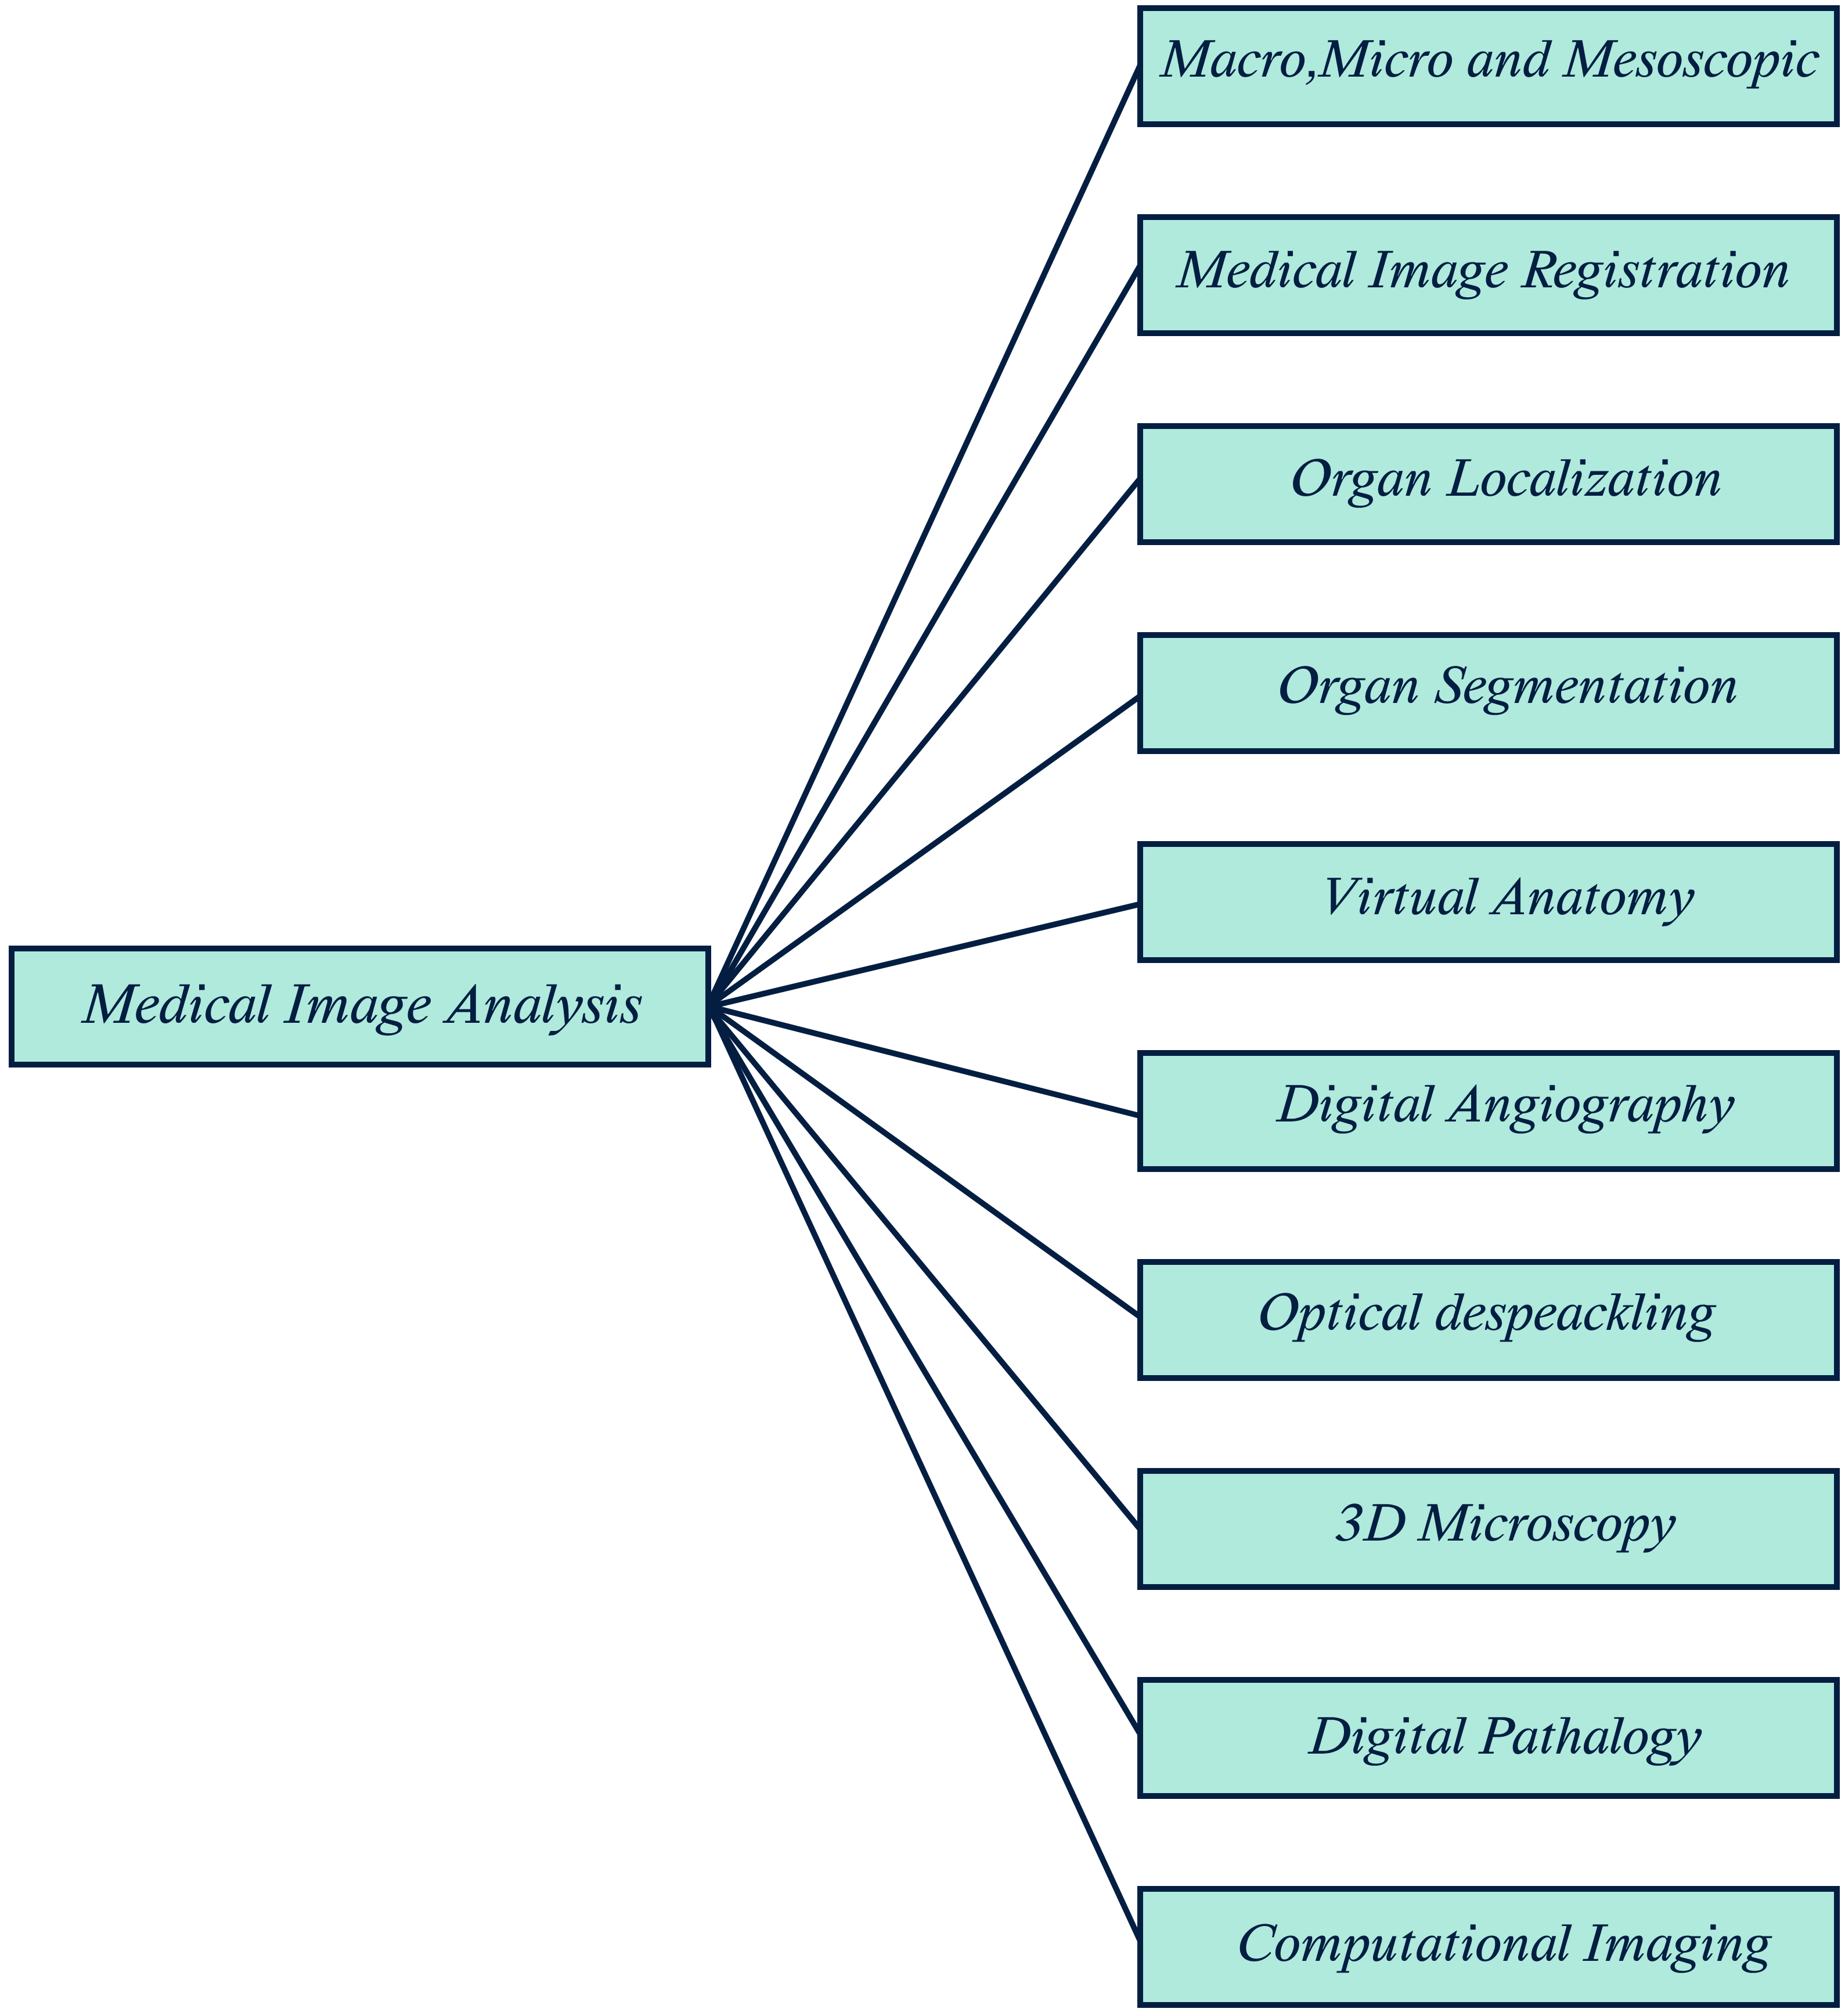
\includegraphics[width=1\columnwidth]{./figures/Fig4.png}
	\caption{Medical image analysis key research(business) areas}
	\label{fig4}
\end{figure}

\section{last 35 years of medical image analysis}
This short review is based on a survey from Duncan and Ayache in January 2000. This era up to 1984 was basically when pattern recognition and analysis were carried on 2D images. Between 1985 and 1991, knowledge-based approaches started, and in that period, we had rule-based analysis and rule-based influencing. From 1992 to 1998, a lot of 3D imaging started into play, and contribution was about storing a more significant amount of data. Silicon fab processes improved process time. For example, nowadays, the whole human body CT could be processed in a couple of minutes, but it took about 24 hours in the past. 

1999 to 2010 was the era of Shallow Reasoning with machine learning, and that is when again you have a lot of computing power. The final period, 2010 until now, is real booming in the field of how neural networks and deep learning was coming up and that is when complex reasoning started. A lot of approaches was developed in this period.

\begin{figure}[htbp]
	%\resizebox{\linewidth}{!}{
	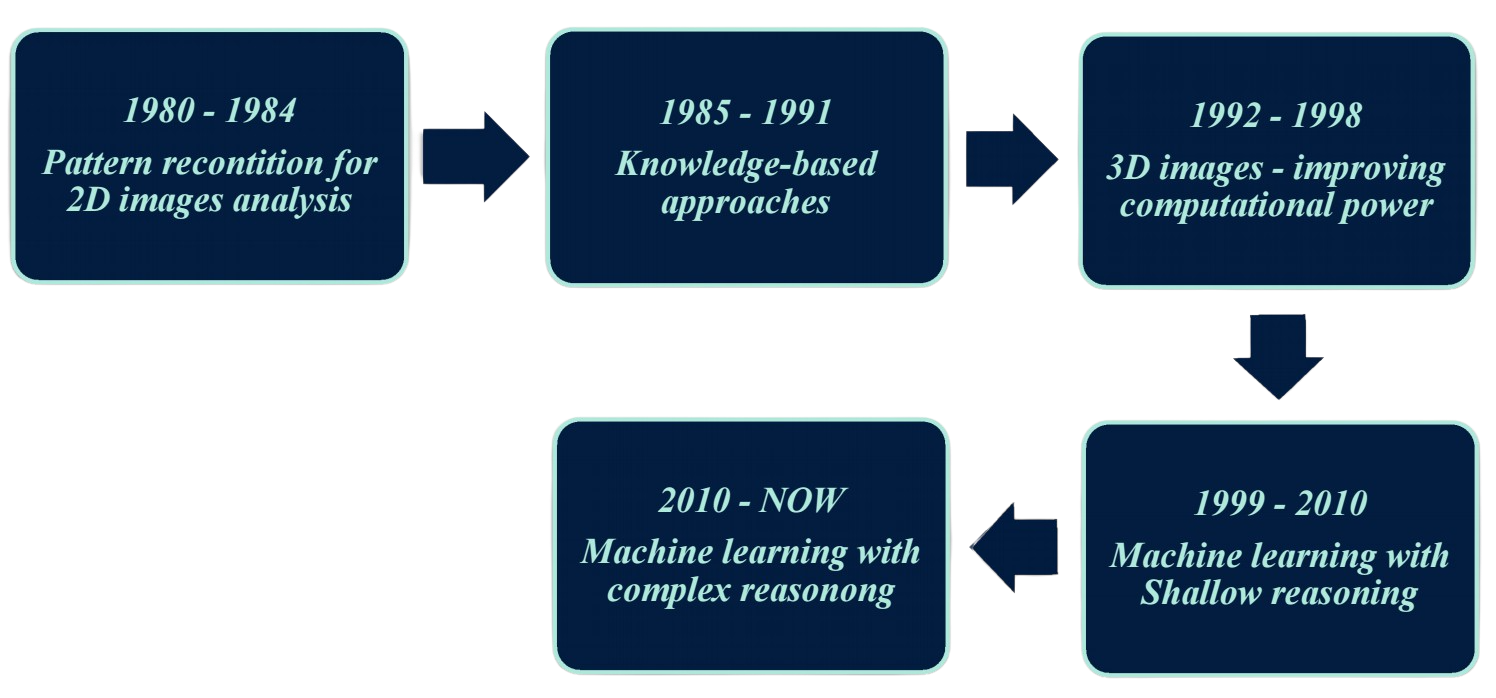
\includegraphics[width=1\columnwidth]{./figures/Fig5.png}
	\caption{Medical image analysis key research(business) areas}
	\label{fig5}
\end{figure}


\section{challenges}

One of the most important challenges for medical image processing is automated detection and classification of breast cancer, and it also called as CAMELYON2017. The next challenge is about prostate lesions segmentation. Then you have the very famous sclerosis from brain MR. The next interesting problem called as M2CAI and this is where we look into interventional videos about surgeries. In other words, M2CAI is modeling and monitoring of computer assisted intervention. The final challenge is ultrasound nerve segmentation.